% !TeX root = ../main.tex
% 原始章节：05-simple-cpu.Rmd

\chapter{简单 LA32R CPU设计}\label{chap:05-simple-cpu}

\section{单周期CPU设计}\label{sec:05-simple-cpu-001}

\subsection{概念介绍}\label{sec:05-simple-cpu-002}

单周期处理器是一种简单的计算机处理器设计方法，其主要特点是每条指令执行所需的时钟周期数是固定的，即每条指令的执行时间相同。单周期处理器的时钟周期包含了所有指令执行所需的所有阶段，如指令取指、指令译码、执行、访存、写回。
所有的指令在同一个时钟周期内按照固定的顺序执行，每个时钟周期执行完整的指令周期。

单周期处理器的优点在于设计相对简单直观，易于理解和实现，常用于计算机体系结构的教学中。由于时钟周期固定，时序控制比较简单。但问题在于每条指令都需花费相同的时钟周期，关键路径较长，导致效率较低，不能充分利用硬件资源。

实际应用中，单周期处理器常用于简单的教学模型和某些低复杂度的嵌入式系统中，例如一些小型控制器或嵌入式设备。在高性能计算机系统中，单周期处理器的使用较少，因为其效率问题和难以处理复杂指令流的特性。

在单周期处理器中，数据通路和控制部件是核心组成部分，负责执行指令并控制处理器的操作。数据通路是处理器中负责执行指令操作的部分，包括寄存器、ALU（算术逻辑单元）、数据存储器（数据缓存或主存）等。其作用是根据指令的需求，执行数据的读取、存储和运算操作。它包含了各种数据传输路径和算术逻辑操作路径，以实现指令的执行功能。

控制部件是处理器中负责解析和执行指令的部分，它根据指令的类型和操作码，生成相应的控制信号来驱动数据通路执行指令操作。其作用是控制部件控制整个处理器的操作流程，包括指令的获取、译码、执行、存储等各个阶段。它决定每个时钟周期内数据通路的工作方式和操作序列。

\subsection{指令介绍}\label{sec:05-simple-cpu-003}

我们主要介绍计算指令、访存指令以及分支跳转指令在单周期处理器中的执行流程，分别以add.w、ld.w、st.w、beq为例。

对于不同指令，其取指、译码环节较为类似。简便起见，假设我们采取哈佛架构的单周期处理器，即将指令存储器与数据存储器分开。指令的执行流程涉及从指令存储器（指令存储器和数据存储器分开存储的结构）中取指令、译码指令、执行操作和结果写回到数据存储器或寄存器的过程。

对于add.w指令，

\begin{enumerate}
\def\labelenumi{\arabic{enumi}.}
\item
  指令取指：控制单元从指令存储器中读取当前指令。指令存储器根据程序计数器（PC，存储当前指令的地址）提供的地址，将指令传送到控制单元。
\item
  指令译码：控制单元对从指令存储器中读取的指令进行解码，确定其操作类型和操作数。对于 add.w 指令，控制单元识别出该指令是进行加法操作。
\item
  操作数获取：控制单元根据指令中的寄存器地址或立即数字段，从寄存器堆中读取操作数。
\item
  执行操作：ALU（算术逻辑单元）接收来自控制单元的操作数，并执行加法运算。ALU 将计算结果存储在临时寄存器中，以供进一步处理。
\item
  结果写回：控制单元将 ALU 计算得到的结果写回到目标寄存器或者数据存储器中。如果 add.w 指令是将两个寄存器相加并将结果存储到第三个寄存器中，则结果会被写回到目标寄存器中。
\end{enumerate}

ld.w指令是从内存取回一个字节的数据后写入通用寄存器rd。对于ld.w指令，其相较add.w指令的差异在于操作数获取与执行操作，具体如下：

\begin{enumerate}
\def\labelenumi{\arabic{enumi}.}
\item
  操作数获取：根据rj寄存器读取操作数，对立即数进行符号拓展。
\item
  访存地址计算：通过ALU将rj寄存器值与符号拓展后的立即数相加，得到访存地址。
\item
  执行操作：根据访存地址从数据存储器中获取结果。
\end{enumerate}

st.w指令是将通用寄存器rd值写入到内存中。对于st.w指令，其差异同样在于操作数获取与执行操作，没有结果写回过程，具体如下：

\begin{enumerate}
\def\labelenumi{\arabic{enumi}.}
\item
  操作数获取：根据rj寄存器读取操作数，对立即数进行符号拓展。
\item
  访存地址计算：通过ALU将rj寄存器值与符号拓展后的立即数相加，得到访存地址。
\item
  执行操作：根据访存地址，将rd寄存器值写入内存。
\end{enumerate}

beq指令是将通用寄存器rj和通用寄存器rd的值进行比较，如果两者相等则跳转到目标地址，否则不跳转。

\begin{enumerate}
\def\labelenumi{\arabic{enumi}.}
\item
  操作数获取，根据rj、rd寄存器读取操作数。
\item
  Target NPC计算：将16位立即数左移两位，然后进行符号拓展
\item
  执行操作：比较rj、rd寄存器值，若相等则将NPC置为Target NPC，不相等则保持不变。
\end{enumerate}

\subsection{数据通路}\label{sec:05-simple-cpu-004}

\begin{figure}[htbp]
  \centering
  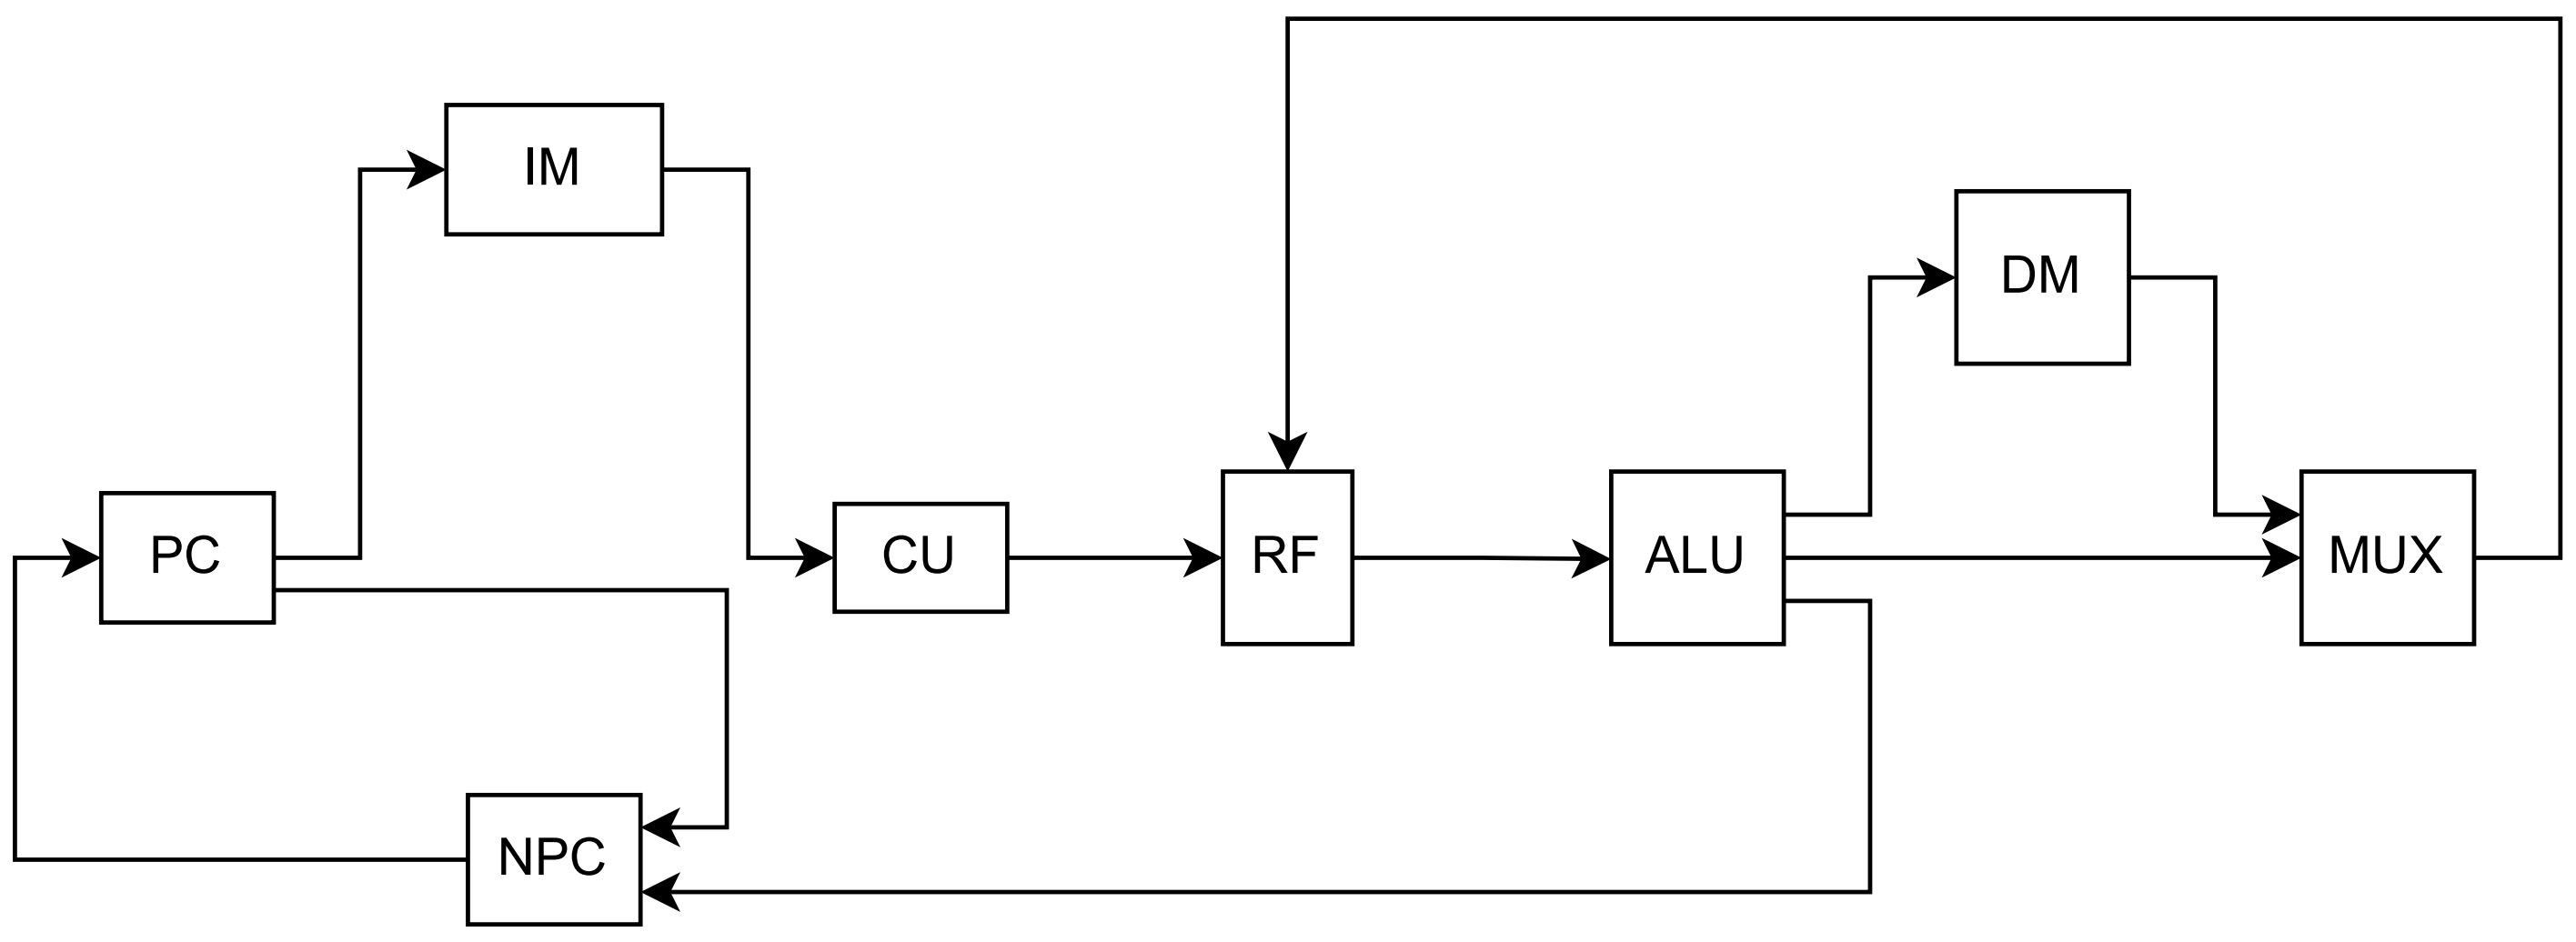
\includegraphics[width=0.75\linewidth]{assets/05/单周期处理器.png}
  \caption{单周期处理器}
  \label{fig:single-cycle-processer}
\end{figure}

如图所示，单周期处理器首先根据PC从指令存储器（IM）中取指，得到指令后进入控制器单元（CU）进行译码，得到控制信号。然后，处理器根据控制信号从寄存器堆（RF）中读取操作数，并将操作数送入ALU。如果为计算指令（如add.w），直接将ALU的结果写回；如果为访存类指令，如ld.w，还会根据ALU计算得到的访存地址从数据存储器（DM）中读值，最后，通过一个多路选择器（MUX）将指令执行结果写回RF。

对于NPC的更新，除了PC+4，还可能有源于ALU的计算结果，下一周期会根据NPC的值更新PC。

\subsection{模块设计}\label{sec:05-simple-cpu-005}

\begin{enumerate}
\def\labelenumi{\arabic{enumi}.}
\tightlist
\item
  程序计数器 (PC)：程序计数器(PC)用于存储当前正在执行的指令的地址，也就是下一条指令的地址。
\end{enumerate}

引脚：

\begin{itemize}
\item
  输入：NPC
\item
  输出：指令地址
\end{itemize}

控制信号：无

\begin{enumerate}
\def\labelenumi{\arabic{enumi}.}
\setcounter{enumi}{1}
\tightlist
\item
  算术逻辑单元 (ALU)：算术逻辑单元(ALU)执行所有的算术和逻辑运算，如加法、减法、逻辑与、逻辑或等。
\end{enumerate}

引脚：

\begin{itemize}
\item
  输入：两个操作数，操作数来源于寄存器文件或立即数。
\item
  输出：运算结果。
\end{itemize}

控制信号：

\begin{itemize}
\item
  ALUOp：指定 ALU 执行的具体操作（例如加法、减法、逻辑运算等）
\item
  ALUSrc：指定 ALU 的一个操作数来源（通常是寄存器文件或者立即数）
\end{itemize}

\begin{enumerate}
\def\labelenumi{\arabic{enumi}.}
\setcounter{enumi}{2}
\tightlist
\item
  数据存储器 (DM)：数据存储器用于存储数据，包括指令执行过程中需要读取或写入的数据。
\end{enumerate}

引脚：

\begin{itemize}
\item
  输入：地址、写入数据。
\item
  输出：从指定地址读取的数据。
\end{itemize}

控制信号：

\begin{itemize}
\item
  MemEn：存储器写使能。
\item
  MemAddr：指定要读取或写入的存储器地址。
\end{itemize}

对于add.w指令，可以设置ALUOp=ADD（对应一个枚举变量），ALUSrc=REG（代表操作数源于寄存器），ALU输入是两个寄存器的值，输出两个寄存器值的和。

对于ld.w指令，可以设置MemEn=0，MemAddr=ALURes(ALU的输出结果)，ALUSrc=IMM(代表操作数源于立即数)，ALUOp=ADD，RegEn(寄存器写使能)，ALU输入时一个寄存器的值和一个立即数，输出是两者之和。

对于st.w指令，可以设置MemEn=1，MemAddr=ALURes，ALUSrc=IMM，ALUOp=ADD，RegEn=0，ALU输入时一个寄存器的值和一个立即数，输出是两者之和。

对于beq指令，可以设置ALUOp=SUB，NPCSrc=Branch(NPC的多路选择控制信号)。

\subsection{指令实现}\label{sec:05-simple-cpu-006}

分类介绍如何给CPU添加指令，说明如何针对不同类型指令添加控制信号、书写控制模块、修改整体设计图。

假设我们已经添加了add.w、ld.w、st.w指令，下面我们将要在现有基础上添加sll.w、ld.b、bl指令。

\begin{itemize}
\tightlist
\item
  sll.w
\end{itemize}

sll.w的数据通路与add.w类似，差别仅在于ALUOp的选择。添加译码信号后，我们将控制信号中的ALUOp选择为SLL，然后在ALU中添加对应的操作，将通用寄存器rj中的数据逻辑左移，移位结果写入通用寄存器rd中。

\begin{itemize}
\tightlist
\item
  ld.b
\end{itemize}

ld.b指令的数据通路与ld.w类似，差别仅在于ld.b是从数据存储器中取回一个字节的数据符号拓展后写入通用寄存器rd，ld.w是从内存取回一个字的数据写入通用寄存器rd。因此，我们将数据从数据存储器中取出后，可以在DM后面添加一个数据后处理器模块，从一个字的数据中截取对应字节，并最终写入RF。

\begin{itemize}
\tightlist
\item
  bl
\end{itemize}

bl指令的一种简单复用现有数据通路的方式是，ALU提供给NPC的反馈信号无条件置高，然后ALU输出PC+4，并最终写回1号通用寄存器r1中。

\section{流水线CPU设计}\label{sec:05-simple-cpu-007}

本节所实现的是不考虑相关冲突的流水线CPU设计，冲突的处理详见后文。

\subsection{概念介绍}\label{sec:05-simple-cpu-008}

流水线CPU是一种通过将指令的执行过程划分为多个阶段来实现并行处理的处理器架构，这种设计有助于提高处理器的吞吐量，从而提高整体性能。下面将详细阐述流水线CPU的划分方式、各个阶段的主要功能、执行特征、以及数据通路和控制部件的概念和作用。

流水线CPU将指令执行过程分为以下五个主要阶段：

\begin{enumerate}
\def\labelenumi{\arabic{enumi}.}
\tightlist
\item
  取指阶段（IF, Instruction Fetch）：负责从内存中读取指令并将其加载到指令寄存器中。
\end{enumerate}

程序计数器（PC）提供指令的地址，然后将指令送入指令缓存，在这一阶段，处理器可能会更新程序计数器以指向下一条指令。

\begin{enumerate}
\def\labelenumi{\arabic{enumi}.}
\setcounter{enumi}{1}
\tightlist
\item
  译码阶段（ID, Instruction Decode）：负责解析指令的操作码和操作数，确定要执行的操作以及需要的寄存器。
\end{enumerate}

从寄存器堆中读取源操作数，将指令的操作码和操作数发送到执行单元准备执行。

\begin{enumerate}
\def\labelenumi{\arabic{enumi}.}
\setcounter{enumi}{2}
\tightlist
\item
  执行阶段（EX, Execution）：负责执行算术或逻辑操作，或者计算内存地址。
\end{enumerate}

执行单元（ALU、乘法器、除法器等）根据译码阶段提供的操作数和指令类型执行操作。对于内存访问指令，此阶段还计算数据的存储地址。

\begin{enumerate}
\def\labelenumi{\arabic{enumi}.}
\setcounter{enumi}{3}
\tightlist
\item
  访存阶段（MEM, Memory Access）：负责访问数据存储器（内存）以读取或写入数据。
\end{enumerate}

如果指令涉及内存操作，这一阶段将数据从内存中读取或将数据写入内存。这一阶段通常涉及数据缓存（Data Cache）的读写操作。

\begin{enumerate}
\def\labelenumi{\arabic{enumi}.}
\setcounter{enumi}{4}
\tightlist
\item
  写回阶段（WB, Write Back）：负责将计算结果写回寄存器堆。
\end{enumerate}

将执行阶段或访存阶段得到的结果写回寄存器堆中的目标寄存器，以便后续指令使用。

流水线各阶段之间通过触发器（Pipeline Registers）实现隔离和同步。这些触发器存储每个阶段的中间数据，使得每个阶段的输出可以在下一阶段使用。例如，从取指阶段到译码阶段的数据通过IF/ID触发器传递，从译码阶段到执行阶段的数据通过ID/EX触发器传递，依此类推。

在现代CPU中，为了提高数据访问的速度，通常会引入同步RAM（Synchronous RAM）。同步RAM在时钟信号的控制下进行数据存取，保证了数据的稳定性和一致性。它能与CPU的流水线操作紧密配合，以实现高效的数据存取和处理。

而在流水线处理器中，数据通路与控制部件的概念与单周期处理器类似。

\subsection{指令介绍}\label{sec:05-simple-cpu-009}

该节介绍LA32R指令中计算指令、分支跳转指令以及访存指令在流水线CPU中的处理流程。

\begin{enumerate}
\def\labelenumi{\arabic{enumi}.}
\tightlist
\item
  计算指令
\end{enumerate}

示例：add.w R1, R2, R3 （将寄存器R2和R3的值相加，并将结果存储到R1中）

\begin{itemize}
\item
  取指阶段：从指令缓存（I-cache）中获取计算指令，并将其送入指令寄存器；更新程序计数器（PC），指向下一条指令。
\item
  译码阶段：解析指令的操作码和操作数；从寄存器堆中读取源寄存器（R2、R3）的值；根据指令类型设置控制信号，指示ALU进行加法操作。
\item
  执行阶段：ALU执行加法操作，将R2和R3的值相加；计算结果准备好用于下一阶段的写回。
\item
  访存阶段：对于纯计算指令，此阶段不涉及内存访问，因此此阶段通常是空闲的。
\item
  写回阶段：将ALU的计算结果写回目标寄存器（R1）。
\end{itemize}

\begin{enumerate}
\def\labelenumi{\arabic{enumi}.}
\setcounter{enumi}{1}
\tightlist
\item
  分支跳转指令
\end{enumerate}

示例：beq R1, R2, LABEL （如果寄存器R1和R2的值相等，则跳转到指定标签的位置）

\begin{itemize}
\item
  取指阶段：从指令缓存中获取分支指令；更新程序计数器（PC），通常指向下一条指令的位置。
\item
  译码阶段：解析分支指令的操作码和目标地址；确定分支条件是否满足（例如，R1是否等于R2）；预测是否发生分支（分支预测机制）。
\item
  执行阶段：计算分支条件（比较R1和R2的值）；如果分支条件满足，计算分支目标地址。
\item
  访存阶段：对于分支指令，此阶段通常不涉及内存操作，除非分支指令本身涉及数据加载。
\item
  写回阶段：分支指令通常不涉及写回阶段，除非是某些特定的分支操作。
\end{itemize}

分支跳转指令可能引发流水线停顿（Pipeline Stalls），因为流水线必须根据分支结果决定是否继续执行下一条指令。

\begin{enumerate}
\def\labelenumi{\arabic{enumi}.}
\setcounter{enumi}{2}
\tightlist
\item
  访存指令
\end{enumerate}

示例：ld.w R1, 0(R2) （从内存地址R2 + 0中加载数据到寄存器R1中）

\begin{itemize}
\item
  取指阶段：从指令缓存中获取访存指令；更新程序计数器（PC），指向下一条指令。
\item
  译码阶段：解析访存指令的操作码和目标寄存器；从寄存器堆中读取源寄存器（R2）的值，计算内存地址；设置控制信号以进行内存访问。
\item
  执行阶段：计算内存地址（R2 + 0）；准备内存访问操作。
\item
  访存阶段：执行内存访问操作，从计算出的内存地址中读取数据（对于加载指令）或将数据写入内存（对于存储指令）。
\item
  写回阶段：将从内存读取的数据写回寄存器（对于加载指令）。
\end{itemize}

对于存储指令（如st.w，将数据写入内存），访存阶段将数据写入内存而不是寄存器。

\subsection{数据通路}\label{sec:05-simple-cpu-010}

在将单周期CPU的数据通路调整为适用于流水线CPU的规范时，需要对数据通路进行更新，以支持流水线阶段的操作。特别地，对于转移指令，需要对程序计数器（PC）的更新机制进行调整。

\begin{itemize}
\item
  添加分支控制单元：引入一个分支控制单元来决定是否发生跳转。该单元根据分支指令的条件和目标地址生成分支控制信号。
\item
  计算分支目标地址：在执行阶段（EX），计算分支目标地址。这个地址通常由指令的偏移量和当前PC值计算得到。
\item
  引入多路选择器：在PC更新路径上添加多路选择器。这个多路选择器用于选择下一条指令的地址。该多路选择器有两个输入：一个是PC的默认递增值（即PC + 4），另一个是分支目标地址。
\item
  控制信号：将分支控制信号连接到多路选择器的控制输入端。根据分支条件是否满足，选择分支目标地址或PC递增值作为下一条指令的地址。
\item
  更新PC：确保PC寄存器的更新通过多路选择器的输出进行。这使得在分支跳转时，PC可以正确地更新到新的指令地址。
\end{itemize}

\subsection{控制信号的设计}\label{sec:05-simple-cpu-011}

在单周期CPU中，整个指令执行过程都在一个时钟周期内完成，控制部件主要负责生成适当的控制信号来指导指令的执行。而在流水线处理器中，指令的执行被分为多个阶段（例如取指阶段、译码阶段、执行阶段、访存阶段和写回阶段），每个阶段都需要控制信号来确保正确的操作顺序和数据流动。

其中，``ready\_go''信号（有时也被称为``ready''信号或``stall''信号）用于协调流水线各阶段之间的操作，确保数据的正确流动和防止数据冒险。这个信号通常指示某一阶段是否准备好接受新的指令或数据，或者是否需要等待。接下来我们来看``ready\_go''信号在不同流水线阶段中的取值及其含义。

\begin{enumerate}
\def\labelenumi{\arabic{enumi}.}
\tightlist
\item
  取指阶段
\end{enumerate}

\begin{itemize}
\tightlist
\item
  ready\_go取值
\end{itemize}

1：表示取指阶段可以从指令缓存中读取新指令。

0：表示取指阶段需要等待，可能是因为前一个阶段的数据还没有准备好，或者因为存在流水线停顿（stall）或数据冒险。

当``ready\_go''信号为1时，取指阶段可以继续进行，从内存或指令缓存中读取下一条指令。如果为0，则取指阶段需要等待，可能需要停顿直到所有前面的流水线阶段都准备好或满足一定的条件。

\begin{enumerate}
\def\labelenumi{\arabic{enumi}.}
\setcounter{enumi}{1}
\tightlist
\item
  译码阶段
\end{enumerate}

1：表示译码阶段可以解码当前指令并生成适当的控制信号和寄存器读取信号。

0：表示译码阶段需要等待，可能是因为前面的取指阶段没有正确读取指令，或者因为需要等待数据或控制信号的准备。

当``ready\_go''信号为1时，译码阶段可以处理当前指令并将其传递给下一个阶段。如果为0，则表示译码阶段必须等待，可能是由于数据依赖或控制信号尚未准备好。

\begin{enumerate}
\def\labelenumi{\arabic{enumi}.}
\setcounter{enumi}{2}
\tightlist
\item
  执行阶段
\end{enumerate}

1：表示执行阶段可以进行算术逻辑运算或地址计算。

0：表示执行阶段需要等待，可能是因为前面的译码阶段未能完成指令解码，或者执行阶段依赖的数据尚未准备好。

当``ready\_go''信号为1时，执行阶段可以进行指令的实际运算。如果为0，则执行阶段必须等待，通常是由于数据冒险、依赖关系未满足或流水线停顿的原因。

\begin{enumerate}
\def\labelenumi{\arabic{enumi}.}
\setcounter{enumi}{3}
\tightlist
\item
  访存阶段
\end{enumerate}

1：表示访存阶段可以从数据缓存中读取或写入数据。

0：表示访存阶段需要等待，可能是因为前面的执行阶段未完成，或者访存操作需要等待数据缓存的响应。

当``ready\_go''信号为1时，访存阶段可以进行内存读写操作。如果为0，则访存阶段需要等待，这可能是由于内存访问的延迟或缓存未准备好。

\begin{enumerate}
\def\labelenumi{\arabic{enumi}.}
\setcounter{enumi}{4}
\tightlist
\item
  写回阶段
\end{enumerate}

1：表示写回阶段可以将计算结果写回到寄存器中。

0：表示写回阶段需要等待，可能是因为前面的访存阶段未能完成，或者写回阶段需要等待数据的准备。

当``ready\_go''信号为1时，写回阶段可以将结果写入寄存器文件。如果为0，则表示写回阶段需要等待，通常是由于数据冒险或访存阶段的延迟。

\section{将CPU核集成到SoC环境中}\label{sec:05-simple-cpu-012}

在System on Chip（SoC）设计中，内存控制器、串口控制器、Flash控制器和网络控制器是核心组件，各自承担不同的功能，并协作以实现系统的整体运作。

\begin{itemize}
\item
  内存控制器：管理SoC中的内存访问，包括RAM和其他类型的内存。它协调数据在处理器和内存之间的读写操作。
\item
  串口控制器：处理串行通信，包括数据的发送和接收。常用于连接外部设备如传感器、调试接口或其他微控制器。
\item
  Flash控制器：管理闪存的读写操作，通常用于存储系统固件、启动代码或用户数据。它保证数据的长期存储和可靠性。
\item
  网络控制器：处理网络接口的通信，如Ethernet，负责数据的接收和发送以实现网络连接。
\end{itemize}

而OpenMegaSoC 提供了 SPI、SDIO、I2S、VGA、Ethernet、UART、CDBUS、I2C 等硬件外设支持。其通过AXI4和AXI4 Lite进行片内互联，地址空间如下：

\begin{enumerate}
\def\labelenumi{\arabic{enumi}.}
\tightlist
\item
  AXI4 外设地址映射
\end{enumerate}

\begin{longtable}[]{@{}
  >{\raggedright\arraybackslash}p{(\linewidth - 4\tabcolsep) * \real{0.6022}}
  >{\raggedright\arraybackslash}p{(\linewidth - 4\tabcolsep) * \real{0.2688}}
  >{\raggedright\arraybackslash}p{(\linewidth - 4\tabcolsep) * \real{0.1290}}@{}}
\toprule\noalign{}
\begin{minipage}[b]{\linewidth}\raggedright
Address Range
\end{minipage} & \begin{minipage}[b]{\linewidth}\raggedright
Device
\end{minipage} & \begin{minipage}[b]{\linewidth}\raggedright
Select Value
\end{minipage} \\
\midrule\noalign{}
\endhead
\bottomrule\noalign{}
\endlastfoot
\texttt{0x00000000\ -\ 0x0FFFFFFF} & Memory Controller & 0 \\
\texttt{0x1C000000\ -\ 0x1C0FFFFF}\newline{}\texttt{0x1D000000\ -\ 0x1D00FFFF} & SPI Device & 1 \\
\texttt{0x1D010000\ -\ 0x1D0FFFFF} & AXI-Lite Device & 2 \\
\texttt{0x1D100000\ -\ 0x1D1FFFFF} & USB Controller & 3 \\
Other Addresses & AXI-Lite Device (Default) & 2 \\
\end{longtable}

\begin{enumerate}
\def\labelenumi{\arabic{enumi}.}
\setcounter{enumi}{1}
\tightlist
\item
  AXI4 Lite 外设地址映射
\end{enumerate}

\begin{longtable}[]{@{}
  >{\raggedright\arraybackslash}p{(\linewidth - 4\tabcolsep) * \real{0.3731}}
  >{\raggedright\arraybackslash}p{(\linewidth - 4\tabcolsep) * \real{0.4478}}
  >{\raggedright\arraybackslash}p{(\linewidth - 4\tabcolsep) * \real{0.1791}}@{}}
\toprule\noalign{}
\begin{minipage}[b]{\linewidth}\raggedright
Address Range
\end{minipage} & \begin{minipage}[b]{\linewidth}\raggedright
Device
\end{minipage} & \begin{minipage}[b]{\linewidth}\raggedright
Select Value
\end{minipage} \\
\midrule\noalign{}
\endhead
\bottomrule\noalign{}
\endlastfoot
\texttt{0x1D010000\ -\ 0x1D03FFFF} & APB Devices (UART, I2C, CDBUS) & 1 \\
\texttt{0x1D040000\ -\ 0x1D04FFFF} & Configuration Registers & 2 \\
\texttt{0x1D050000\ -\ 0x1D05FFFF} & Ethernet Controller & 3 \\
\texttt{0x1D060000\ -\ 0x1D06FFFF} & Interrupt Controller & 4 \\
\texttt{0x1D070000\ -\ 0x1D07FFFF} & SD Controller & 5 \\
\texttt{0x1D0A0000\ -\ 0x1D0AFFFF} & JPEG Controller & 6 \\
\texttt{0x1D0B0000\ -\ 0x1D0BFFFF} & I2S Controller-0（DMA） & 7 \\
\texttt{0x1D0C0000\ -\ 0x1D0CFFFF} & I2S Controller-1（GEN） & 8 \\
\texttt{0x1D0D0000\ -\ 0x1D0DFFFF} & VGA Controller & 9 \\
Other Addresses & SRAM Controller (Default) & 0 \\
\end{longtable}

而为了接入OpenMegaSoC，你需要使得自己的CPU对外保持AXI4接口，接口具体定义如下：

% 代码语言：BookVerilog
\begin{CodeBlock}[language=BookVerilog]
module mycpu_mega_top(
  input         clock,
  input         reset,
  input         awready,
  output        awvalid,
  output [31:0] awaddr,
  output [2:0]  awprot,
  output        awid,
  output        awuser,
  output [7:0]  awlen,
  output [2:0]  awsize,
  output [1:0]  awburst,
  output        awlock,
  output [3:0]  awcache,
  output [3:0]  awqos,
  input         wready,
  output        wvalid,
  output [31:0] wdata,
  output [3:0]  wstrb,
  output        wlast,
  output        bready,
  input         bvalid,
  input  [1:0]  bresp,
  input         bid,
  input         buser,
  input         arready,
  output        arvalid,
  output [31:0] araddr,
  output [2:0]  arprot,
  output        arid,
  output        aruser,
  output [7:0]  arlen,
  output [2:0]  arsize,
  output [1:0]  arburst,
  output        arlock,
  output [3:0]  arcache,
  output [3:0]  arqos,
  output        rready,
  input         rvalid,
  input  [1:0]  rresp,
  input  [31:0] rdata,
  input         rlast,
  input         rid,
  input         ruser,
  input  [7:0]  ext_int,
  output        global_reset
);
\end{CodeBlock}

\section{SoC环境下的CPU功能仿真与调试}\label{sec:05-simple-cpu-013}

为了简化仿真环境下的调试难度，eula-env中使用的仿真SoC（EulaSoC）仅包含CPU、RAM、Confreg三个设备，且片内通过AXI4总线进行互联。具体而言，CPU对外外一束AXI4总线接口，通过AXI4 Demux分为三束。对应地址空间为\texttt{0xbfaf0000\textasciitilde{}0xbfb00000}、\texttt{0x1faf0000\textasciitilde{}1fb00000}以及\texttt{0x0\textasciitilde{}0x100000000}中的其他地址空间。其中，前两束AXI4总线接口会再通过AXI4 Mux合并为一束，连接Confreg，另外一束AXI4总线接口会连接RAM。

EulaSoC中CPU的对外接口与OpenMegaSoC中CPU的对外接口保持一致，因此可延续上述接入方式。

\section{处理流水线冲突}\label{sec:05-simple-cpu-014}

\subsection{冲突类型介绍}\label{sec:05-simple-cpu-015}

在处理器中，可能存在三种冲突：

\begin{enumerate}
\def\labelenumi{\arabic{enumi}.}
\item
  资源冲突：发生在多个指令需要同一硬件资源时，例如两个指令同时访问寄存器或ALU（算术逻辑单元）。
\item
  数据冲突：发生在一条指令依赖于另一条指令的结果时，例如指令A的结果被指令B使用，但指令A还未完成。
\item
  控制冲突：发生在指令流的顺序由于分支指令而改变时，例如条件跳转指令使得处理器无法确定下一条执行指令的地址。
\end{enumerate}

\subsection{通过阻塞技术解决冲突}\label{sec:05-simple-cpu-016}

在现代处理器中，为了提高性能和避免数据冲突，处理器设计者采用了多种技术，包括阻塞技术。下面介绍了如何通过阻塞解决四种主要的数据冲突：写后写（WAW）、写后读（WAR）、读后写（RAW）、读后读（RAR）。

\begin{enumerate}
\def\labelenumi{\arabic{enumi}.}
\tightlist
\item
  写后写（WAW, Write After Write）：WAW数据冲突发生在两条指令都试图向同一个寄存器写入数据时。如果指令B试图在指令A完成写操作之前写入同一个寄存器，可能会导致数据的不确定性。
\end{enumerate}

阻塞技术可以通过在指令B写入前插入``气泡''或暂停指令执行来解决此问题。具体做法如下：

\begin{itemize}
\item
  检测冲突： 确定是否有两条指令要写入同一寄存器。
\item
  插入气泡： 在指令B的执行前插入气泡，等待指令A完成其写操作。
\end{itemize}

\begin{enumerate}
\def\labelenumi{\arabic{enumi}.}
\setcounter{enumi}{1}
\tightlist
\item
  写后读（WAR, Write After Read）：WAR数据冲突发生在一条指令试图读取某寄存器的值，而另一条指令随后写入该寄存器。如果写操作在读操作之前完成，可能导致读取到过时的数据。
\end{enumerate}

阻塞技术通过插入气泡来解决WAR冲突，确保读取操作在写入操作之前完成。具体方法包括：

\begin{itemize}
\item
  检测冲突： 确定是否有一条指令正在读取某个寄存器，同时另一条指令计划写入该寄存器。
\item
  插入气泡： 将写操作推迟，直到读取操作完成，确保数据一致性。
\end{itemize}

\begin{enumerate}
\def\labelenumi{\arabic{enumi}.}
\setcounter{enumi}{2}
\tightlist
\item
  读后写（RAW, Read After Write）：RAW数据冲突发生在一条指令试图读取一个寄存器的值，而另一条指令尚未完成对该寄存器的写入。如果读取操作在写入操作之前执行，会读取到过时的或不完整的数据。
\end{enumerate}

阻塞技术可以通过在读取操作前插入气泡来解决RAW冲突。具体步骤包括：

\begin{itemize}
\item
  检测冲突： 识别是否有一条指令需要读取一个寄存器，而另一条指令尚未完成对该寄存器的写入。
\item
  插入气泡： 暂停读取操作，直到写操作完成，确保读取到最新的值。
\end{itemize}

\begin{enumerate}
\def\labelenumi{\arabic{enumi}.}
\setcounter{enumi}{3}
\tightlist
\item
  读后读（RAR, Read After Read）：RAR数据冲突发生在两条指令都试图读取同一个寄存器。通常，RAR冲突不会引起问题，因为读取操作不改变寄存器的值，因此这种冲突比较少见。
\end{enumerate}

通常情况下，不需要特别的阻塞措施来解决RAR冲突，因为读取操作不会互相干扰。但在某些高性能处理器中，可能会通过预测和调度技术优化执行顺序。

\subsection{通过前递技术解决冲突}\label{sec:05-simple-cpu-017}

为了减少阻塞并提高处理器的执行效率，可以引入数据前递（data forwarding）通路。数据前递是一种技术，通过直接将指令的结果传递给依赖于它的后续指令，避免了不必要的等待和气泡插入。具体做法如下：

\begin{enumerate}
\def\labelenumi{\arabic{enumi}.}
\tightlist
\item
  检测数据依赖
\end{enumerate}

处理器需要识别哪些指令对前一指令的结果有数据依赖。这包括检测RAW（读后写）和WAW（写后写）冲突。处理器通过内置的数据冒险检测单元来完成这项任务。

\begin{enumerate}
\def\labelenumi{\arabic{enumi}.}
\setcounter{enumi}{1}
\tightlist
\item
  实现数据前递通路
\end{enumerate}

在流水线阶段添加前递路径：在流水线的各个阶段（如执行阶段、写回阶段），添加逻辑电路用于将指令的结果直接传递给需要这些结果的指令。对于复杂的处理器设计，可能需要多个前递通路来支持不同流水线阶段之间的数据传递。例如，从执行阶段到执行阶段，或者从写回阶段到执行阶段。

\begin{enumerate}
\def\labelenumi{\arabic{enumi}.}
\setcounter{enumi}{2}
\tightlist
\item
  调整控制逻辑
\end{enumerate}

更新控制单元：控制单元需要更新以支持数据前递，确保在依赖数据的指令中正确配置前递通路。管理数据转发：设计控制逻辑来处理转发数据的选择和路由，确保数据在正确的时间被转发到正确的指令。

\begin{enumerate}
\def\labelenumi{\arabic{enumi}.}
\setcounter{enumi}{3}
\tightlist
\item
  处理数据前递的限制
\end{enumerate}

解决数据前递延迟：确保数据前递通路的延迟最小化，以减少因转发延迟引起的性能瓶颈。管理资源竞争：处理器需要管理多个指令同时请求前递数据的情况，确保资源合理分配。

假设指令A在ALU中执行并写入寄存器R1，而指令B需要读取寄存器R1的值。如果没有数据前递，指令B必须等待指令A完成写操作。但是，通过数据前递，指令A执行的结果可以直接传递给指令B，避免了额外的等待时间，从而减少了阻塞。
